%% LyX 2.3.1 created this file.  For more info, see http://www.lyx.org/.
%% Do not edit unless you really know what you are doing.
\documentclass[12pt,english,letterpaper]{kuthesis}
\usepackage{mathptmx}
\renewcommand{\sfdefault}{lmss}
\renewcommand{\ttdefault}{lmtt}
\usepackage[T1]{fontenc}
\usepackage[utf8]{inputenc}
\usepackage{geometry}
\geometry{verbose,tmargin=1in,bmargin=1in,lmargin=1in,rmargin=1in}
\setcounter{secnumdepth}{3}
\setcounter{tocdepth}{3}
\usepackage{color}
\usepackage{babel}
\usepackage{url}
\usepackage{graphicx}
\usepackage{setspace}
\usepackage{esint}
\usepackage[authoryear]{natbib}
\doublespacing
\usepackage[unicode=true,
 bookmarks=true,bookmarksnumbered=false,bookmarksopen=false,
 breaklinks=true,pdfborder={0 0 0},pdfborderstyle={},backref=false,colorlinks=true]
 {hyperref}
\hypersetup{pdftitle={University of Kansas Thesis Template},
 pdfauthor={Anonymous},
 pdfsubject={A Thesis},
 urlcolor={black},citecolor={black},allcolors={black}}

\makeatletter

%%%%%%%%%%%%%%%%%%%%%%%%%%%%%% LyX specific LaTeX commands.
\providecommand{\LyX}{\texorpdfstring%
  {L\kern-.1667em\lower.25em\hbox{Y}\kern-.125emX\@}
  {LyX}}
%% Because html converters don't know tabularnewline
\providecommand{\tabularnewline}{\\}

%%%%%%%%%%%%%%%%%%%%%%%%%%%%%% User specified LaTeX commands.


%used to align decimals in tables according to APA style
\usepackage{dcolumn}
\usepackage{booktabs}

% Set the title and author info
\title{Please Read the Abstract}
\author{Abstract Writer}

% Following is OPTIONAL list of previous degrees earned. 
% If there are more than 5 or so, then title pagelayout may become too crowded,
% depending on the number of committee members. 
\priorcreds{B.A. Philosophy, Harvard, 1999}{M.A. English, Oxford 2000}{M.A. History, Johnson County Community College, 2005}
% It is acceptable to delete \priorcreds if it is not desired on title page


\dept{Department of People who read Abstracts}
\degreetitle{Doctor of Philosophy}
\papertype{Dissertation} %or Thesis (Choose whatever word you want to put on p.2)

%% Committee member names are required for the title page. We make space
%% for as many as 7 members, with various roles/titles.
%% It is required to have 7 entries, even if some are empty for committee and role
\committee{Member Name 1}{Member Name 2}{Member Name 3}{Member Name 4}{Member 5 has a long name}{Member 6}{}
\role{Chairperson}{Co-Chair}{}{The One Who Never Answers Email}{}{External Reviewer}{}
%At Most 7 members allowed, last here is blank on purpose to demonstrate
%flexibility

%%BOTH dates must be included. 
\@printd@testrue
\datedefended{July 02, 2019}
\dateapproved{August 06, 2019}

%% These settings are now in the kuthesis.cls file, but users are free
% to customize. listings has great documentation online
%% When listings are used, break lines
%\lstset{
 %    breaklines=true,  % sets automatic line breaking
 %    breakindent=2em,
 %    breakatwhitespace=true,  % sets if automatic breaks should
 %   breakautoindent=true
%}

\@ifundefined{showcaptionsetup}{}{%
 \PassOptionsToPackage{caption=false}{subfig}}
\usepackage{subfig}
\makeatother

\usepackage{listings}
\renewcommand{\lstlistingname}{\inputencoding{latin9}Listing}

\begin{document}
\begin{romanpages}

\maketitle

\begin{abstractlong}

Hopefully, you are reading ``ku-thesis.pdf''. If you are reading
a file with some other name, then there's been a goof up. This document
is produced by the LaTeX compiler ``pdflatex''. The file collection
needed to reproduce this document is named ``KU-thesis-20190201.zip''
(the date changes from time to time, of course). The Web home for
this project is \url{https://crmda.ku.edu/latex}\footnote{Previous versions have been offered at \url{http://pj.freefaculty.org/guides/Computing-HOWTO/KU-thesis}. }.
That site will always point at the newest edition and there should
also be a copy in the Electronic Thesis Webpages pages hosted by the
office of the Graduate Dean.

You will love using \LaTeX{} to prepare your thesis. The power to keep
content structured, with a systematic framework for cross references
among figures, tables, equations, and sections, will significantly
improve your quality of life. This will be much better than using
an ordinary ``text editor.''

Well, that's all well and good. But what \emph{is} this? There are
three kinds of files.
\begin{enumerate}
\item The LaTeX class file, \texttt{kuthesis.cls}. That's necessary, you
need that to produce a thesis.
\item The example document, \texttt{thesis-ku}, which can serve as a template
for student projects.
\item A layout file for the LyX editor, \texttt{kuthesis.layout}. You need
that if you want to use LyX to edit your thesis documents.
\end{enumerate}
This is the Spring 2019 revision template. The only major change this
time is the introduction of a new environment, ``chapterabstract''.
This was a frequently requested feature. Before that, the other major
changes in ``\texttt{kuthesis.cls}'' concerned the display of a
student's previous degrees and the members of the thesis committee.
The class file allows students to list as many as 7 committee members,
each with their own titles and roles. The size of the names of the
chapters is now slightly reduced (from the LaTeX \texttt{\textbackslash Huge}
to \texttt{\textbackslash Large}). The ``prior credits'' enhancement
was prepared by Amber Roberts-Graham of the KU Office of the Graduate
Dean. This allows the inclusion of previously obtained degrees on
the title page.

How to use these files.

\textbf{Step 1. Study the features in this document.} Please read
through this Abstract. It is intended to be readable, pleasant, welcoming
and helpful. The PDF you are reading was created by compiling \texttt{thesis-ku.tex}. 

\textbf{Step 2. Inspect the LaTeX source code.}

There are some special features that will become apparent once you
look at the LaTeX source code. The \texttt{thesis-ku} document is
the ``master'' document. The separate chapters are in separate folders.
It is possible to work on one chapter at a time, and compile just
that chapter, or it is possible to compile the whole thing by compiling
the master document.

In \texttt{thesis-ku}, we have included as many bells and whistles
as possible so that users can see how the different features can be
put to use. We have a BibTeX bibliography, graphs, equations, cross
references, table of contents, and all of the other interesting features.

In 2017, we included support for hyperlinks in the PDF output. We
checked with the KU Graduate Dean's office and they said there is
no policy prohibiting the use of hyperlinks, but there is also no
guarantee from the dissertation hosting institution that they will
be allowed in submitted documents. We believe there is not too much
danger here, this feature is easy to turn off if need be. Also, it
is not entirely clear what color the links must be inside the document,
so we take a conservative step here of making the links black, so
they appear as simple text. The default settings for the \texttt{hyperref}
package, which we have altered, caused ugly pink links with gross
looking boxes around them. Users can change the link color to blue.
It is fairly easy to see how this can be done in the document preamble.
Colors can be revised in the hyperref options. Look for ``\texttt{urlcolor=\{black\},
citecolor=\{black\}, allcolors=\{black\}''} and think of Henry Ford's
famous comment, ``You can have a car in any color you like, as long
as its black.'' 

\textbf{Step 3. Try to compile the thesis-ku document!} Before you
edit this (and put your name on it), please \textbf{STOP}! Recompile
this document exactly as it is. This will test your LaTeX setup. Until
you reproduce the PDF you are reading now, you are not ready to start
making changes. People often come forward with questions and our first
question for them is ``did you compile (without error) \texttt{thesis-ku.tex}?''
Until we hear those people say ``yes'', we are generally unable
to help with their revised documents. That's the only way we will
know if your \LaTeX{} setup is ready to go. 

Windows \& Mac users: it is \emph{necessary to extract }the project
folder. Do not use the file manager's ``zip preview'' feature. Extract
the files, or else nothing at all will work.

When you extract the folder, do not rearrange or rename files yet.
Don't change chapter directories. All of these things work together.
Test our setup before altering it.

The file \texttt{kuthesis.cls} is the class file. The document should
compile if that file is in the same directory as the document \texttt{thesis-ku}.
However, there may be warnings from your LaTeX editor that ``\texttt{kuthesis.cls}''
is not available because it is not ``installed'' into your LaTeX
distribution. For testing, ignore the warning. For the long term,
consider installing \texttt{kuthesis.cls}. 

\emph{If you have used \LaTeX}, you will find this more or less self
explanatory. There's a \LaTeX{} file ``\texttt{thesis-ku.tex}''.
It is a ``master'' document, it links together the content of several
files. Compile that with \texttt{\textbf{pdflatex}}. The class file
that makes this go, ``\texttt{kuthesis.cls}'', is saved in the current
working directory. 

\emph{If you have never used \LaTeX}, we will tell you how to compile
this document. But, before you try, can we give you a warning: \emph{please
don't make writing your dissertation your first \LaTeX{} project}.
Start with some simpler example documents. Write some letters to your
loved ones, experiment a little bit. In the KU Center for Research
Methods and Data Analysis, there are occasional workshops for people
who want to get started with \LaTeX . There are many ``how to get
started with \LaTeX '' websites. Ours is \url{http://crmda.ku.edu/latex}.

If you have never used LaTeX before, a good way to start is with the
editor named LyX. Instead of editing the ``raw'' LaTeX file \texttt{thesis-ku.tex},
use LyX to edit \texttt{thesis-ku.lyx}. There is a separate section
below about using LyX. LyX will warn you when you open \texttt{thesis-ku.lyx
because the cls file seems unavailable. Don't worry about that.}

\textbf{Step 4. Revise thesis-ku: Write a Dissertation.}

If you are using a \LaTeX{} editor like TexShop, Tex Works, or \TeX{}
Studio, the source document you need to edit and compile is ``\texttt{thesis-ku.tex}.''
If you plan to use \LyX , the place to start is by opening ``\texttt{thesis-ku.lyx}''
in \LyX 's editor. LyX versions change over time. We are using LyX-2.2.3
at the moment.

The first user customization is to insert your name and the names
of some committee members. The document has a top section called a
``preamble.'' (If using \LyX , click the Document menu, then Settings,
and look down). In the preamble, you will find the following block:

\begin{singlespace}
\noindent \inputencoding{latin9}
\begin{lstlisting}[basicstyle={\small},tabsize=2]
% Set the title and author info
\title{Please Read the Abstract}
\author{Abstract Writer}
% Following is OPTIONAL list of previous degrees earned. 
% If there are more than 5 or so, then title pagelayout 
% may become too crowded,
% depending on the number of committee members. 
\priorcreds{B.A. Philosophy, Harvard, 1999}{M.A. English, Oxford 2000}{M.A. History, Johnson County Community College, 2005}
% It is acceptable to delete \priorcreds if it is not desired 
% on title page
\dept{Department of People who read Abstracts}
\degreetitle{Doctor of Philosophy}
\papertype{Dissertation}%or Thesis 
% (Choose whatever word you want to put on p.2)
% Committee member names are required for the title page. 
% We make space for as many as 7 members, with various 
% roles/titles.
% It is required to have 7 entries, even if some are empty
% for committee and role
\committee{Member Name 1}{Member Name 2}{Member Name 3}{Member Name 4}{Member 5 has a long name}{Member 6}{}
\role{Chairperson}{Co-Chair}{}{The One Who Never Answers Email}{}{External Reviewer}{}
\end{lstlisting}
\inputencoding{utf8}
\end{singlespace}

Here you see the most important template updates for October, 2015.
We have enhanced \texttt{\textbackslash committee} and \texttt{\textbackslash role}
environments. We allow as many as 7 committee members and each one
can have a different role. Why provide all of this luxury? There were
unexpected requests from students. Users asked for a secondary title
``Co-Chair'' for member 2. Then they wanted to change the title
of the first member to ``Lead Chair''. Then they wanted to add a
the third Co-Chair, and so forth. 

Now we accommodate those requests by leaving blank spots for up to
seven committee members and seven roles. It is vital for you to leave
the blank place holders \{\}. This example document shows some funny
titles, we do that only to prove it is possible. Generally, there
is only a Chair, possibly a Co-Chair. 

The other thing to change is the date section. Lower in the preamble,
you should see a place to insert some dates. Fix the dates:

\begin{singlespace}
\noindent \inputencoding{latin9}
\begin{lstlisting}[showstringspaces=false,tabsize=2]
%BOTH dates must be included.  
\@printd@testrue
\datedefended{July 02, 2019} 
\dateapproved{August 06, 2019}
\end{lstlisting}
\inputencoding{utf8}
\end{singlespace}

\noindent Originally, we told students ``just write those dates in
by hand, like we did back in the olden days.'' That was incorrect,
they need to be typeset into the document. 

After you make those changes in the preamble, compile the document.

\textbf{How to Configure your LaTeX Distribution with kuthesis.cls}

I wish we had packaged \texttt{kuthesis.cls} into an official LaTeX
distribution package so that it could be easily installed by your
distribution. We did not do that, however, and so it is up to you
to place a copy of \texttt{kuthesis.cls} in the right spot\texttt{.}
This is not truly necessary. Programs like pdflatex will find \texttt{kuthesis.cls}
if you have it in the same directory as the document. If you want
to use kuthesis.cls for several documents, the best approach is to
install ``\texttt{kuthesis.cls}'' into your \LaTeX{} file structure.
That is generally an easy process, but it is different on every type
of computer. The CRMDA staff has recently prepared a guide for this,
entitled ``How Users can Install \LaTeX{} packages without Help from
System Administrators'' (\url{https://crmda.ku.edu/guide-32-latex_config}).
The gist of this is as follows:

\begin{enumerate}
\item Copy ``\texttt{kuthesis.cls}'' into a directory in your \LaTeX{}
distribution. Usually (almost always), you will find a directory component
that ends in ``tex/latex'' and you can put kuthesis.cls in there.
The only puzzle is finding the right place, and that's why you should
review our guide.
\item Run ``texhash'' or to make the \LaTeX{} distribution take notice
of your new file. On Mac and Linux systems, open a terminal and run
``\texttt{sudo texhash}'' to get this done as the administrator.
\end{enumerate}
\textbf{How to Get Started on this with \LyX}

This document with \LyX ! It will work. LyX is a pleasant-to-use editor,
it can protect you from some of the details that ordinary \LaTeX{}
will present. \LyX{} is free to use on all major computing platforms,
including Linux, Macintosh, and Windows. \LyX{} can be downloaded at
\url{http://www.lyx.org}. To make this work, LaTeX programs are also
needed. 
\begin{enumerate}
\item Mac users: install the ``MacTeX'' package (\url{https://www.tug.org/mactex}). 
\item Linux users: install your distribution's version of TeXLive or install
the TeXLive files from the TeXLive website (\url{https://www.tug.org/texlive})
. 
\item Windows Users: The LyX website offers 2 choices, a LyX-only package
and an ``installer bundle'' that includes LyX along with a small
subset of the MikTeX LaTeX distribution. This installs just a small
subset of MikTeX and pieces can be separately downloaded when needed.
In Fall, 2016, we had some difficulties during a LaTeX workshop because
the MikTeX package server was unavailable. As a result, we have been
migrating away from MikTeX (and the LyX installer bundle) to use TeXLive
for Windows (\url{https://www.tug.org/texlive}). That's a big 2GB
package like MacTeX, after that we install the LyX program. If you
choose the MikTeX setup instead, it will usually be fine, but users
often complain that LyX seems to ``freeze'' when it downloads new
MikTeX components.
\end{enumerate}
If you install a LaTeX distribution and LyX, then you can open the
file ``thesis-ku.lyx''. Warnings–\emph{not errors}–appear. 

\begin{tabular}{cc}
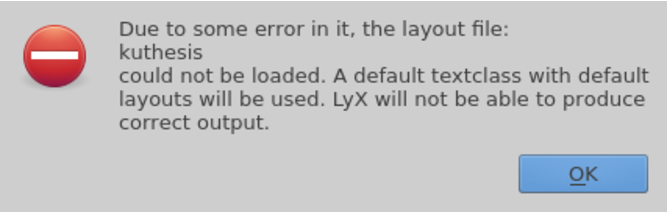
\includegraphics[width=2in]{images/lyx-nolayout} & 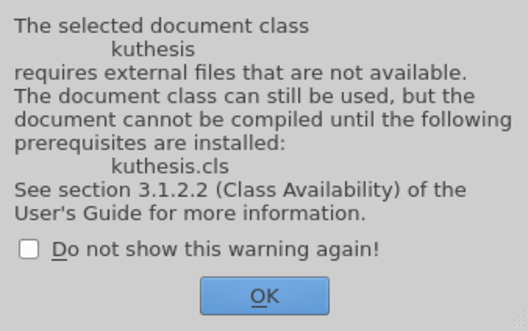
\includegraphics[width=2.5in]{images/lyx-noclsfile}\tabularnewline
\end{tabular}

We will explain how to eliminate these warnings, but you can ignore
them for the moment. Just click ``OK'' 5 or 6 times. After that,
you will find that the dissertation document can be compiled (even
though there were horrible scary warnings). To compile the document,
either click on the ``googly eyes'' icon in the toolbar or use the
keyboard shortcut ``Ctl-R''. If your system has a PDF viewer installed
and LyX can find it, all will be well. We are warned by Windows 10
users that Microsoft has made the Web browser ``Edge'' the default
PDF viewer and that does not work well with LyX. We recommend installing
the PDF viewer Sumatra (\url{https://www.sumatrapdfreader.org/free-pdf-reader.html})
and then using the Windows configuration to set Sumatra as the default
PDF viewer.

Why does \LyX{} work? When the user asks \LyX{} to preview the PDF output,
a two step process happens behind the scenes. A file named ``\texttt{thesis-ku.tex}''
is created in a temporary directory, and then \texttt{\textbf{pdflatex}}
is asked to turn that into a PDF document. \LyX{} will then send the
PDF output to a PDF viewer, such as Yapp, Evince or Acrobat.

How to silence the LyX warnings.

\noindent \textbf{1. See previous subsection ``How to Configure your
LaTeX Distribution with kuthesis.cls'' Do that!}

\noindent \textbf{2. Set a LyX layout file in your use LyX configuration. }

\noindent In essence, copy our file ``\texttt{stylefiles/kuthesis.layout}''
into the user configuration.

Finding the correct user configuration folder is the hard part.

On~Linux, copy \texttt{kuthesis.layout} into the user HOME folder,
under ``\texttt{.lyx/layouts}''. 

On~Windows, there is a hidden AppData directory inside the user's
home folder. How to find it? Run \LyX . A window should appear with
a row of pull down menus at the top. Choose Tools/Preferences. Change
something trivial, then close the menu. That will force \LyX{} to create
a user folder. Then search inside your user directory for a key word
such as ``lyxrc.defaults''. Probably, searching for ``{*}lyx{*}''
will be sufficient. In MS Windows 7, I found the LyX settings were
saved in \inputencoding{latin9}
\begin{lstlisting}
C:\Users\pauljohn\AppData\Roaming\lyx212\layouts
\end{lstlisting}
\inputencoding{utf8}Caution: The AppData folder is hidden/concealed and, in order to find
it in Windows Explorer, it is necessary to change the folder options
to NOT hide protected files and folders. 
\begin{description}
\item [{On~Macintosh~OS~X,}] we recently followed the same ``change
a setting, then search'' procedure. The answer was ``/Users/pauljohn/Library/Application
Support/\LyX -2.1/layouts''. Documentation for OS X indicates that
Apple has followed the Microsoft policy of hiding this folder, so
the person who uses the Finder will have to change some preferences
to show the directory.
\end{description}
\noindent \textbf{3. Let LyX find your changes.}

\noindent In LyX, find the pull down menu item Tools -> Reconfigure.
Then close LyX and restart.

\noindent \textbf{4. Spell checking}

We notice that LyX is not, by default, configured to do spell-checking
as you type. To turn on the spell checker, use the pull down menu
\texttt{Tools} -> \texttt{Preferences} -> \texttt{Language Settings}
-> \texttt{Spellchecker}. One must choose a program to serve as the
``Spellchecker engine'' and then click ``Spellcheck Continuously''.
The Spellchecker engine I use in Ubuntu Linux is called Enchant. I
expect you will find one in your operating system, or can find one.
If not, we may have to ask Mr. Google for help.

\textbf{Other friendly advice.}

\emph{Compile Early, Compile Often}

The truly bad part of using \LaTeX{} is that the errors and warnings
are, generally, not understandable. They are not understandable to
me and I've been using \LaTeX{} for about 20 years. I mean, well, they
are simply too abstract. Too complicated. If you insert an illegal
character, such as an ``\_'' in a \LaTeX{} box, the document will
fail with this unhelpful message

\begin{singlespace}
\noindent \inputencoding{latin9}
\begin{lstlisting}[breaklines=true,tabsize=2]
Missing $ inserted.
Missing $ inserted.
Missing } inserted.
Extra }, or forgotten \endgroup.
...
I've inserted a begin-math/end-math symbol since I think you left one out. Proceed, with fingers crossed.
\end{lstlisting}
\inputencoding{utf8}
\end{singlespace}

\noindent At best, the message will point to the line you inserted
to cause the problem, but often the \LaTeX{} system cannot guess where
your mistake is, it can only say something is wrong. The best way
to defend yourself: \textbf{\textit{Compile Early, Compile Often}}\textbf{.
}Don't make a lot of changes without trying to compile. It is easy
to insert a feature that breaks the document. Compile often so you
know when things have gone wrong. 

\emph{Use a Version Management System!}

If this is an important project, please consider installing Git or
some other version management program. It is difficult to avoid clutter
if you have to rename your file every day. I see user directories
full of files named, ``my\_diss.lyx'', ``my\_diss.2.lyx'', ``my\_diss\_final.lyx'',
``my\_diss\_rejected.lyx'' and so forth. It is very difficult to
keep old and new versions straight unless you use a version manager.
A version manager will handle that for you. You will just have one
file ``my\_diss.lyx'' and you will have the ability to compare old
and new snapshots. The CRMDA has a more-or-less comprehensive, yet
easy to follow guide for Git, ``Git it Together'' (\url{http://crmda.ku.edu/git-help}).

I urge you to keep your \LaTeX{} document in Git so you can make frequent
commits and it will be easy to step back in time. This is one reason
why you should work on separate chapters, so if you break something,
then you are more likely to find your mistakes.

\emph{KU requires that fonts be compiled with the final result}

The pdflatex compiler will insert fonts when it compiles the document.
However, there is a ``gotcha''. If you create illustrations (say,
with R or Matlab) or sub-documents separately in PDF, and you forget
to embed the fonts with them, then the KU Graduate Dean's office is
likely to reject your thesis. When a PDF is included within this document,
\texttt{pdflatex} does not check to see if fonts are embedded in those
PDFs. It assumes they are as you want them; fonts for those included
files are not automatically inserted by pdflatex. When a graph, for
example, is created in R and exported to PDF, it will not include
the font encodings by default. It is possible to add those encodings.
Little details like this come up from time to time and we make note
of them in \url{https://crmda.ku.edu/latex-help}.

\emph{If you need help, ask, but please understand }

I don't have as much time as I would like to help users. I want you
to use \LaTeX . I think doing anything else is finger painting. I've
watched 20 MA and PhD theses written with this template and I know
a bright student will succeed and be happy with the result. If you
have a laptop computer and you want to show me some errors, I can
give you 5 or 10 minutes. But not much more... 

CRMDA offers some workshops and I teach graduate courses in which
we show how to use \LaTeX . If you find something wrong with kuthesis.cls,
I will be glad to try to fix it. 

I don't have time/ability to answer a million email questions about
\LaTeX{} or \LyX . If you are stuck on a tough problem, I may be able
to help, but if I have to exert myself, you should know I expect you
to give me a t-shirt and/or add me to the acknowledgments in your
dissertation. (I'm not joking on that.) I spent about 20 hours helping
a KUMC student fix his LaTeX and he assured me I'll get a big discount
on treatment for any liver illnesses I may endure in the future. (I'm
joking about that.) I did get a medical center license plate holder,
though.

Paul Johnson <pauljohn@ku.edu>

Prof. Political Science \& Director, Center for Research Methods and
Data Analysis

2019-02-01

And that's the end of the abstract.

\end{abstractlong}

\begin{acknowledgementslong}
%%if you want a "quote" environment for acknowledgements,
%% use acknowledgements instead of acknowledgementslong

I would like to thank all of the little people who made this thesis
possible. Sleepy, Dopey, Grumpy, you know who you are.

\end{acknowledgementslong}

\tableofcontents{}

\listoffigures

\listoftables

\end{romanpages}

%% LyX 2.3.1 created this file.  For more info, see http://www.lyx.org/.
%% Do not edit unless you really know what you are doing.
\documentclass[12pt,english]{kuthesis}
\usepackage{mathptmx}
\usepackage[T1]{fontenc}
\usepackage[utf8]{inputenc}
\usepackage{geometry}
\geometry{verbose,tmargin=1in,bmargin=1in,lmargin=1in,rmargin=1in}
\setcounter{secnumdepth}{3}
\setcounter{tocdepth}{3}
\setlength{\parskip}{\smallskipamount}
\setlength{\parindent}{0pt}
\usepackage{graphicx}
\usepackage[authoryear]{natbib}

\makeatletter

%%%%%%%%%%%%%%%%%%%%%%%%%%%%%% LyX specific LaTeX commands.
%% Because html converters don't know tabularnewline
\providecommand{\tabularnewline}{\\}

%%%%%%%%%%%%%%%%%%%%%%%%%%%%%% User specified LaTeX commands.
%%\usepackage{latexsym}
\usepackage{graphicx}

%%\usepackage{psfig}
%%\usepackage{color}

%%%%%%%%%%%%%%%%%%%%%%%%%%%%%% User specified LaTeX commands.
\usepackage{ragged2e}
\RaggedRight
%\setlength{\parindent}{1.5 em}

\makeatother

\usepackage{babel}
\begin{document}

\chapter{The Only Chapter}

\begin{chapterabstract}
Initial Attempt at Using University Package to Write my Initial Drafted Documentation from Microsoft Word
\end{chapterabstract}

\section{Draft}

Some text.

\end{document}


\global\long\def\bibname{References}%

\bibliographystyle{apalike2}
\bibliography{Biblio/allcites}


\appendix

\chapter{My Appendix, Next to my Spleen}

There could be lots of stuff here

\end{document}
